% Options for packages loaded elsewhere
\PassOptionsToPackage{unicode}{hyperref}
\PassOptionsToPackage{hyphens}{url}
%
\documentclass[
  12pt,
]{article}
\usepackage{amsmath,amssymb}
\usepackage{lmodern}
\usepackage{setspace}
\usepackage{iftex}
\ifPDFTeX
  \usepackage[T1]{fontenc}
  \usepackage[utf8]{inputenc}
  \usepackage{textcomp} % provide euro and other symbols
\else % if luatex or xetex
  \usepackage{unicode-math}
  \defaultfontfeatures{Scale=MatchLowercase}
  \defaultfontfeatures[\rmfamily]{Ligatures=TeX,Scale=1}
  \setmainfont[Scale=MatchLowercase]{Lato}
  \setmathfont[]{Fira Math}
\fi
% Use upquote if available, for straight quotes in verbatim environments
\IfFileExists{upquote.sty}{\usepackage{upquote}}{}
\IfFileExists{microtype.sty}{% use microtype if available
  \usepackage[]{microtype}
  \UseMicrotypeSet[protrusion]{basicmath} % disable protrusion for tt fonts
}{}
\usepackage{xcolor}
\usepackage[margin=1.3in]{geometry}
\usepackage{longtable,booktabs,array}
\usepackage{calc} % for calculating minipage widths
% Correct order of tables after \paragraph or \subparagraph
\usepackage{etoolbox}
\makeatletter
\patchcmd\longtable{\par}{\if@noskipsec\mbox{}\fi\par}{}{}
\makeatother
% Allow footnotes in longtable head/foot
\IfFileExists{footnotehyper.sty}{\usepackage{footnotehyper}}{\usepackage{footnote}}
\makesavenoteenv{longtable}
\usepackage{graphicx}
\makeatletter
\def\maxwidth{\ifdim\Gin@nat@width>\linewidth\linewidth\else\Gin@nat@width\fi}
\def\maxheight{\ifdim\Gin@nat@height>\textheight\textheight\else\Gin@nat@height\fi}
\makeatother
% Scale images if necessary, so that they will not overflow the page
% margins by default, and it is still possible to overwrite the defaults
% using explicit options in \includegraphics[width, height, ...]{}
\setkeys{Gin}{width=\maxwidth,height=\maxheight,keepaspectratio}
% Set default figure placement to htbp
\makeatletter
\def\fps@figure{htbp}
\makeatother
\setlength{\emergencystretch}{3em} % prevent overfull lines
\providecommand{\tightlist}{%
  \setlength{\itemsep}{0pt}\setlength{\parskip}{0pt}}
\setcounter{secnumdepth}{5}
\newlength{\cslhangindent}
\setlength{\cslhangindent}{1.5em}
\newlength{\csllabelwidth}
\setlength{\csllabelwidth}{3em}
\newlength{\cslentryspacingunit} % times entry-spacing
\setlength{\cslentryspacingunit}{\parskip}
\newenvironment{CSLReferences}[2] % #1 hanging-ident, #2 entry spacing
 {% don't indent paragraphs
  \setlength{\parindent}{0pt}
  % turn on hanging indent if param 1 is 1
  \ifodd #1
  \let\oldpar\par
  \def\par{\hangindent=\cslhangindent\oldpar}
  \fi
  % set entry spacing
  \setlength{\parskip}{#2\cslentryspacingunit}
 }%
 {}
\usepackage{calc}
\newcommand{\CSLBlock}[1]{#1\hfill\break}
\newcommand{\CSLLeftMargin}[1]{\parbox[t]{\csllabelwidth}{#1}}
\newcommand{\CSLRightInline}[1]{\parbox[t]{\linewidth - \csllabelwidth}{#1}\break}
\newcommand{\CSLIndent}[1]{\hspace{\cslhangindent}#1}
\usepackage{booktabs}
\usepackage{longtable}
\usepackage{array}
\usepackage{multirow}
\usepackage{wrapfig}
\usepackage{float}
\usepackage{colortbl}
\usepackage{pdflscape}
\usepackage{tabu}
\usepackage{threeparttable}
\usepackage{threeparttablex}
\usepackage[normalem]{ulem}
\usepackage{makecell}
\usepackage{xcolor}
\ifLuaTeX
  \usepackage{selnolig}  % disable illegal ligatures
\fi
\IfFileExists{bookmark.sty}{\usepackage{bookmark}}{\usepackage{hyperref}}
\IfFileExists{xurl.sty}{\usepackage{xurl}}{} % add URL line breaks if available
\urlstyle{same} % disable monospaced font for URLs
\hypersetup{
  pdftitle={Why Ain't Evidentialists Rich?},
  pdfauthor={Anon},
  hidelinks,
  pdfcreator={LaTeX via pandoc}}

\title{Why Ain't Evidentialists Rich?}
\author{Anon}
\date{2022-08-24}

\begin{document}
\maketitle

\setstretch{1.4}
There is a familiar complaint against Causal Decision Theory (CDT) that goes back to the modern origins of decision theory in the 1970s. Here is a recent version of it due to Ahmed and Price (2012). (I've slightly changed some of the wording, but otherwise this argument is quoted from page 16 of their paper.)

\begin{enumerate}
\def\labelenumi{\arabic{enumi}.}
\tightlist
\item
  In Newcomb problems, the average returns to one-boxing exceed that to two-boxing.
\item
  Everyone can see that (1) is true.
\item
  Therefore one-boxing foreseeably does better than two-boxing. (by 1, 2)
\item
  Therefore Causal Decision Theory (CDT) is committed to the foreseeably worse option for anyone facing Newcomb's problem.
\end{enumerate}

Here's what they, and many other proponents of Evidential Decision Theory (EDT) say follows from 4.

\begin{quote}
The point of the argument is that if everyone knows that the CDT-irrational strategy will in fact do better on average than the CDT-rational strategy, then it's rational to play the CDT-irrational strategy. (Ahmed and Price 2012, 17)
\end{quote}

This is what Lewis (1981) called the ``Why Ain'cha Rich'' argument, and what following Bales (2018) I'll call the WAR argument. I'm going to argue the last step of the WAR argument doesn't follow. Or, at the very least, that proponents of EDT cannot coherently say that it follows. For there are several cases where EDT foreseeably does worse than CDT. This section will go over three of them.

\hypertarget{example-one---split-newcomb}{%
\section{Example One - Split Newcomb}\label{example-one---split-newcomb}}

This game takes place over three rounds.

\begin{enumerate}
\def\labelenumi{\arabic{enumi}.}
\tightlist
\item
  At stage one, the human player chooses Play or Exit. If they choose Out, player gets 5 and demon gets 1. If they choose In, we move onto stage two.
\item
  At stage two, demon chooses Left or Right, and this choice is announced.
\item
  At stage three demon and the player simultaneously choose either Up or Down. Demon is very good at predicting what player's choices will be, and indeed at stage two they were already very good at making such a prediction. And Demon wants to use these predictive powers to get as high a payoff as possible, and this is common knowledge.
\end{enumerate}

If Demon chose Left at stage two, stage three involves the game in table \ref{tab:left-anti-war}. But if Demon chose Right at stage two, stage three involves the game in table \ref{tab:right-anti-war}. If you'd prefer it as a game tree, it is presented in figure \ref{fig:first-anti-war}.

\renewcommand{\arraystretch}{1.3}   
\begin{table}

\caption{\label{tab:left-anti-war}The left hand side of Split Newcomb.}
\centering \vspace{6pt}
\begin{tabular}[t]{>{}r>{}c>{}c}

\textbf{} & \textbf{PU} & \textbf{PD}\\

\textbf{U} & 2, 1 & 4, 0\\
\textbf{D} & 1, 0 & 3, 3\\

\end{tabular}
\end{table}

\renewcommand{\arraystretch}{1.3}   
\begin{table}

\caption{\label{tab:right-anti-war}The right hand side of Split Newcomb.}
\centering \vspace{6pt}
\begin{tabular}[t]{>{}r>{}c>{}c}

\textbf{} & \textbf{PU} & \textbf{PD}\\

\textbf{U} & 12, 4 & 14, 0\\
\textbf{D} & 11, 0 & 13, 2\\

\end{tabular}
\end{table}

\begin{figure}
\centering
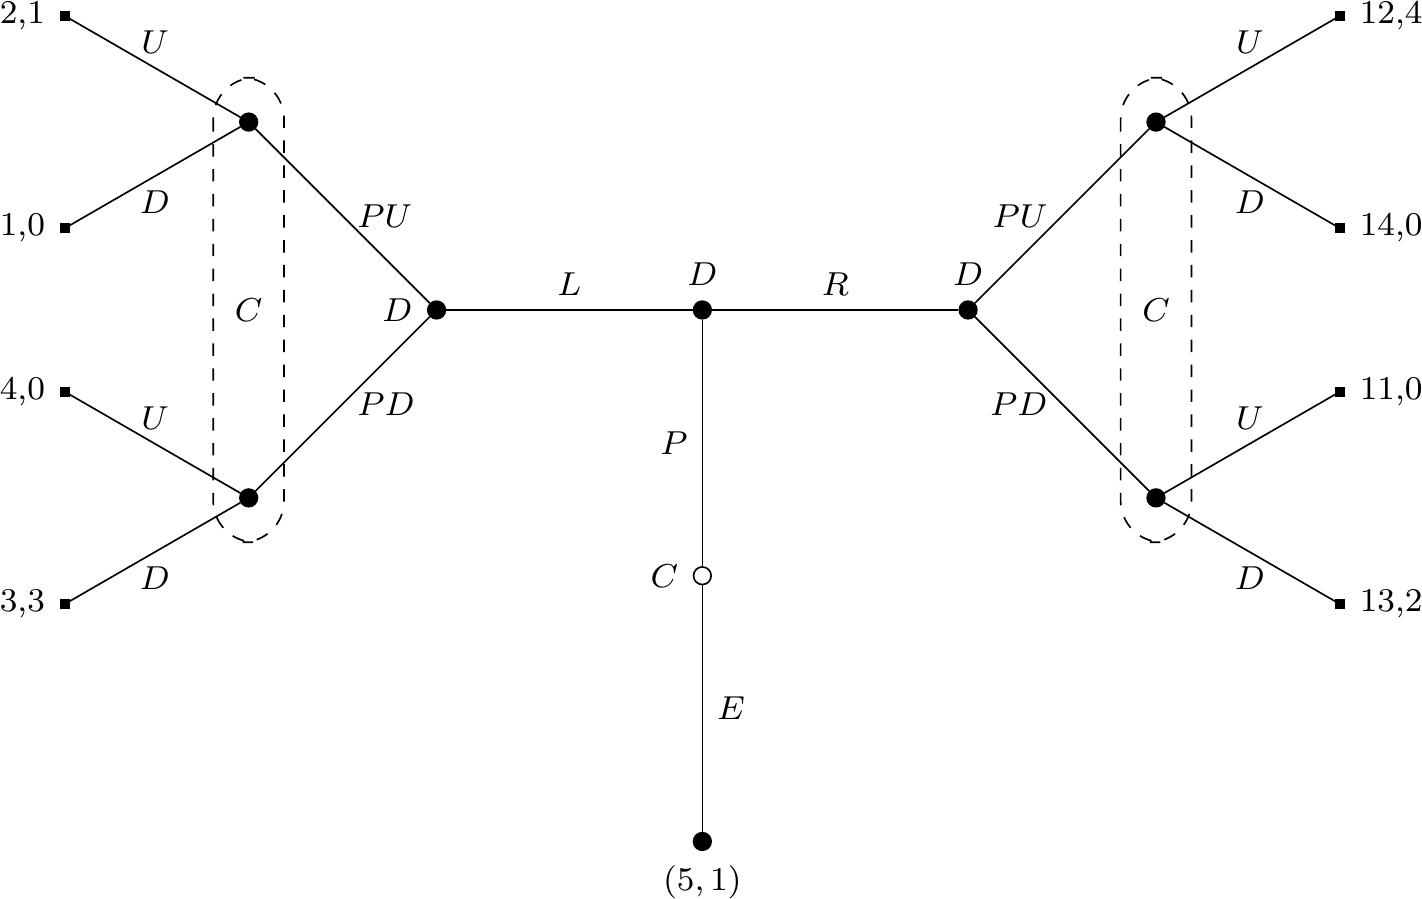
\includegraphics{war-on-war_files/figure-latex/first-anti-war-1.png}
\caption{\label{fig:first-anti-war}Tree Diagram of the Split Newcomb Game}
\end{figure}

We start at the hollow node in the middle, and Chooser (here denoted as `C') either goes up by Playing, or goes down by Exiting. Then Demon moves Left or Right. Then Demon moves again, making a prediction. But this second move isn't revealed to Chooser, which is why on either side Chooser's nodes are in an information set. That's to say, Chooser chooses Up or Down knowing whether Demon has gone Left or Right, but not knowing whether Demon has predicted Up or Down. And then we get the payoffs.

Whether Demon goes Left or Right, the CDTer will choose Up, and the EDTer will choose Down. Either choice Chooser faces is a fairly straightforward Newcomb Problem. In both sub-games Up causally dominates Down, but Down will get a higher return if you assume, as we did assume, that demon mostly makes correct predictions.

So at stage two, Demon will know that if the person facing them is an EDTer, they will get a return of 3 from Left and 2 from Right. (They'll end up in the Down-Down cell either way.) So they will rationally choose Left. On the other hand, if the person facing them is a CDTer, they will get a return of 1 from Left and 4 from Right. (They'll end up in the Up-Up cell either way.) So they will rationally choose Right. And everything in this paragraph can be deduced by a rational player at stage 1.

So at stage one, a CDTer will know that if they Play, they expect to get 12 (the game will go Right then Up-Up), and if they Exit, they know they'll get 5. So they'll Play. But an EDTer will know that if they Play, they expect to get 4 (the game will go Left then Down-Down), and if they Exit, they know they'll get 5. So they'll Exit.

The result of all this is that the CDTer will get 12, and the EDTer will get 5. So the CDTer will predictably do better than the EDTer. Indeed, the EDTer will voluntarily choose at stage one to take a lower payout than the CDTer ends up with. This seems bad for EDT, at least if we think that predictably ending up with a lower outcome is bad.

Now you might object that this is because at stage two Demon chooses to treat the EDTer differently to how they treat the CDTer. I don't really agree for two reasons, though I'm not sure either of these reasons work. (Hence the second and third examples that are about to come.) One is that Demon isn't trying to harm the EDTer; they are just trying to maximise their return. It so happens that EDT is such an impermissive theory that it doesn't allow for any flexibility, and Demon, knowing this, is forced to take choices that are bad for EDT, and indeed worse for Demon than if they ended up at Right-Up-Up. But this isn't Demon's fault; it's the fault of EDT being so impermissive. The other reason is that Demon does not in fact make any choices that hurt the EDTer. The EDTer should expect that Demon will in fact make such choices, in response to their theory, but that's not quite the same thing. The only player who moves at all in the EDT version of the game is Chooser. So it's a little hard to say this is just a case where the EDTer is harmed by Demon's malicious choices.

I think those responses work, but as I said, they don't even fully convince me. And I'm normally more sympathetic to my arguments than others are. So let's look at a different example, one where Demon doesn't have these variable payouts.

\hypertarget{coinssignals}{%
\section{Example Two - Coins and Signals}\label{coinssignals}}

This example is a version of a signaling game of the kind introduced by Lewis (1969). And in particular it's a version of the broadly adversarial kinds of signaling games that are central to the plot of Cho and Kreps (1987). Again, it will involve three stages.

At the first stage a fair coin is flipped, and the result shown to Chooser, but not to Demon. At the second stage, Chooser will choose Up or Down, and the choice will be publicly announced. At the third stage, Demon will try to guess what the coin showed. Demon knows the payoff table I'm about to show you, and is arbitrarily good at predicting Chooser's strategy. That is, Demon can make accurate predictions of the form ``If Heads, Chooser will make this choice, and if Tails, they will make that choice.'' The payoffs to each player are a function of what happens at each of the three steps, and are given by table \ref{tab:payoffs-demon-coin}.

\begin{table}

\caption{\label{tab:payoffs-demon-coin}Payoffs for the coins and signals game.}
\centering \vspace{6pt}
\begin{tabular}[t]{>{}c>{}c>{}c>{}c>{}c}

\textbf{Coin} & \textbf{Chooser} & \textbf{Demon} & \textbf{Chooser Payoff} & \textbf{Demon Payoff}\\

H & U & U & 40 & 1\\
H & U & T & 400 & 0\\
H & D & U & 0 & 1\\
H & D & T & 0 & 0\\
T & U & U & 40 & 0\\
T & U & T & 28 & 1\\
T & D & U & 28 & 0\\
T & D & T & 36 & 1\\

\end{tabular}
\end{table}

\begin{figure}
\centering
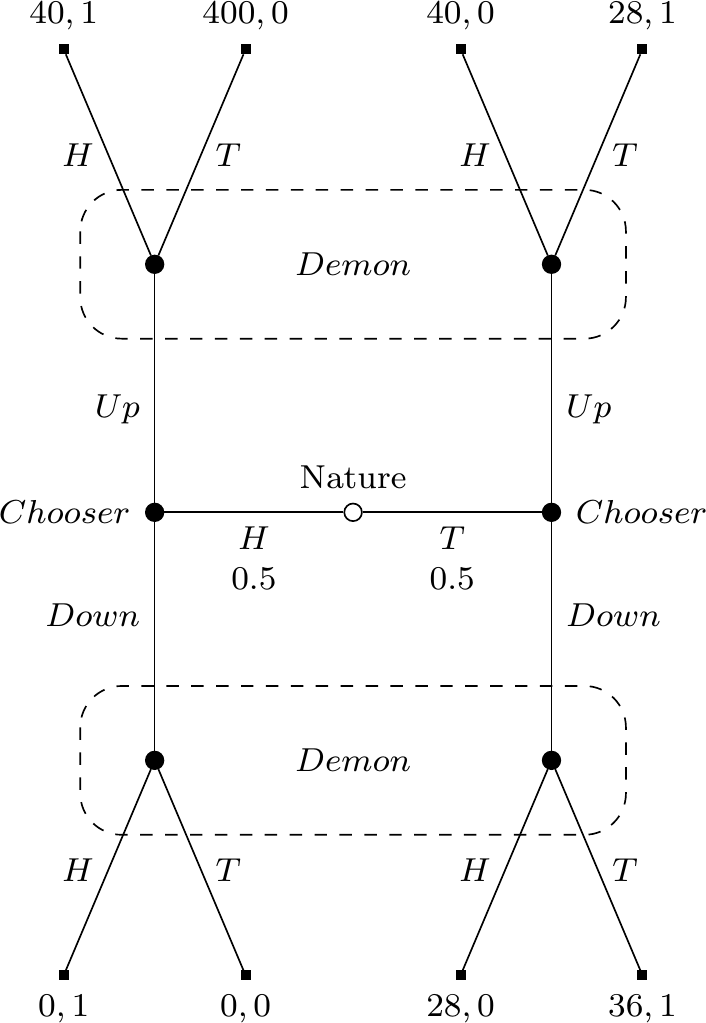
\includegraphics{war-on-war_files/figure-latex/second-anti-war-1.png}
\caption{\label{fig:second-anti-war}Tree Diagram of the Coins and Signals Game}
\end{figure}

Figure \ref{fig:second-anti-war} shows the game they are playing in tree form. Demons's payoffs are just as you'd expect - they get rewarded iff they figure out how the coin landed. Chooser's payoffs are more complicated, but the big thing to note is they get the biggest rewards if they manage to play Up while Demon makes an incorrect prediction.

One last thing to stipulate about Demon before we analyse the game. If Demon predicts Chooser will do one thing if Heads and another if Tails, they will use the information from Chooser's choice to make their guess about how the coin landed. But if they predict Chooser will say the same thing whether the coin landed Heads or Tails, they won't know how the coin landed, and will flip their own coin to make a guess. So in that case it will be 50/50 whether Demon says Heads or Tails.

Onto the analysis. It should be fairly clear that if the coin lands Heads, the human should say Up. The worst possible return from Up is 40, the best possible return from Down is 0. So that's what both a CDTer and an EDTer would do, and hence what Demon would predict that they will do.

So what happens if the coin lands Tails? Given Demon will predict Up if Heads, we can work out the value of Up and Down if Tails to the EDTer. If they play Up, Demon will predict that, and hence Demon will flip a coin to choose Heads or Tails. So they have a 50/50 shot at getting either 40 or 28, and so their expected return is 34. If they play Down, Demon will predict that, and hence Demon will say Tails, and they will get a return of 36. Since 36 \textgreater{} 34, they will play Down if Tails.

That's the unique solution to the game for the EDTer. They play Up if Heads, Down if Tails. Demon can figure out that they'll do this, so will correctly guess what the coin showed. And they will get 40 if the coin landed Heads, and 36 if it landed Tails, for an expected return of 38.

What should the CDTer do? This is a somewhat interesting problem, and I don't think all causal decision theorists will agree on it. My preferred version of CDT does not issue a verdict on this case. It says that it is permissible to do what EDT does, and it's permissible to play the strategy of Up no matter what. The latter is a very lucrative strategy. Given they are doing the same thing whatever the coin says, Demon won't get any information by predicting their strategy and observing their play. So Demon will simply flip their own coin, and hence lines 1, 2, 5 and 6 of the table are all equally likely to appear. So if Chooser plays this strategy, they are equally likely to get a return of 40, 400, 40 or 28, for an overall expected return of 127. And this is much higher than the 38 the EDTer is expected to receive. By changing the payout on line 2 of the table, we can make the gap in expected returns be arbitrarily large.

Now you might object that I haven't shown, and in fact don't believe, that CDT must play this strategy. So I haven't shown that CDT does better in this case than EDT.I don't think that matters much. The point of the WAR is to refute a theory, and if the EDTer does foreseeably worse than one kind of Chooser, that should be enough to refute them. But just in case you think that we need a case where CDT clearly does better than EDT, I'll include one last example.

\hypertarget{example-three---coins-and-newcomb}{%
\section{Example Three - Coins and Newcomb}\label{example-three---coins-and-newcomb}}

This is just like Example Two, with one twist. If the game goes Tails, Down, Tails, then we don't immediately end the game and make payouts to the players. Instead we play another game, with a familiar structure, and the payouts shown in table \ref{tab:third-anti-war}. As always, Demon is really good at predicting Chooser's play, and Chooser's payouts are listed first in every cell. (I'm not going to include a tree here, because it is more confusing than helpful.)

\renewcommand{\arraystretch}{1.3}   
\begin{table}

\caption{\label{tab:third-anti-war}The payouts after tails–down–tails in coins and Newcomb.}
\centering \vspace{6pt}
\begin{tabular}[t]{>{}r>{}c>{}c}

\textbf{} & \textbf{PU} & \textbf{PD}\\

\textbf{U} & 20, 1 & 40, 0\\
\textbf{D} & 16, 0 & 36, 1\\

\end{tabular}
\end{table}

The EDTer will think they'll get 36 from this game, so the example will be just like Example Two. And the EDTer will play Up if Heads, Down if Tails, for an expected return of 38.

But if Chooser follows CDT, then they will think that if the game gets to this stage, they'll get 20. So now they think that in the original game, Up dominates Down no matter whether the coin lands Heads or Tails. So now they will definitely play Up no matter what, and get an expected return of 127.

\hypertarget{why-the-examples-matter}{%
\section{Why The Examples Matter}\label{why-the-examples-matter}}

This paper is very much not an argument against EDT; instead, it's part of a war on WAR. The point of the first example is that any theory whatsoever is subject to a WAR argument. That's because for any theory whatsoever, you can construct pairs of choices like Left and Right, where the theory says to take choices that lead Demon to preferring to go Left. So for any theory whatsoever, or at least any theory that is consequentialist in the sense popularised by Hammond (1988), there is an example where the theory leads to worse returns. So any consequentialist theory is subject to an objection by WAR. It's the paradigm of an over-generating objection.

There is perhaps something a bit interesting about the second example, though it isn't a problem especially for EDT. What makes the second example work is that Chooser is in a situation that rewards unpredictability, and EDT is predictable in all cases that don't involve ties. Indeed, any theory that is predictable in cases that don't involve ties will be subject to an WAR-style objection from cases like this. So we'll end with two clear lessons from the cases. The first is that EDTers can't endorse WAR-style objections, since there is such an objection to their theory. The second is that everyone should worry about WAR-style objections backfiring; the examples here can be easily generalised to tell against most theories of decision.

\hypertarget{references}{%
\section*{References}\label{references}}
\addcontentsline{toc}{section}{References}

\hypertarget{refs}{}
\begin{CSLReferences}{1}{0}
\leavevmode\vadjust pre{\hypertarget{ref-AhmedPrice2012}{}}%
Ahmed, Arif, and Huw Price. 2012. {``Arntzenius on `Why Ain'cha Rich?'.''} \emph{Erkenntnis} 77 (1): 15--30. \url{https://doi.org/10.1007/s10670-011-9355-2}.

\leavevmode\vadjust pre{\hypertarget{ref-Bales2018}{}}%
Bales, Adam. 2018. {``Richness and Rationality: Causal Decision Theory and the WAR Argument.''} \emph{Synthese} 195 (1): 259--67. \url{https://doi.org/10.1007/s11229-016-1214-x}.

\leavevmode\vadjust pre{\hypertarget{ref-ChoKreps1987}{}}%
Cho, In-Koo, and David M. Kreps. 1987. {``Signalling Games and Stable Equilibria.''} \emph{The Quarterly Journal of Economics} 102 (2): 179--221. \url{https://doi.org/10.2307/1885060}.

\leavevmode\vadjust pre{\hypertarget{ref-Hammond1988}{}}%
Hammond, Peter J. 1988. {``Consequentialist Foundations for Expected Utility.''} \emph{Theory and Decision} 25: 25--78. \url{https://doi.org/10.1007/BF00129168}.

\leavevmode\vadjust pre{\hypertarget{ref-Lewis1969a}{}}%
Lewis, David. 1969. \emph{Convention: A Philosophical Study}. Cambridge: Harvard University Press.

\leavevmode\vadjust pre{\hypertarget{ref-Lewis1981e}{}}%
---------. 1981. {``Why Ain'cha Rich?''} \emph{No{û}s} 15 (3): 377--80. \url{https://doi.org/10.2307/2215439}.

\end{CSLReferences}

\end{document}
